\documentclass[11pt]{article}

%\usepackage{sfheaders}        %% Chap/Sec headers in Helvetica
\usepackage[margin=2cm]{geometry}
\usepackage{epigraph}         %% section quotations
\setlength{\epigraphwidth}{.95\textwidth}
\renewcommand{\epigraphsize}{\normalsize}
\setlength{\epigraphrule}{0pt}
\setlength{\beforeepigraphskip}{.2\baselineskip}
\setlength{\afterepigraphskip}{0pt}
\usepackage[obeyspaces]{url}  %% URLs and pathnames
\usepackage[]{hyperref}
\usepackage{graphicx}


\usepackage[comma]{natbib}
\renewcommand{\bibname}{References}
\bibliographystyle{abbrvnat-apa}  % this includes URLs

%opening
\title{Quotes on Statistics, Data Visualization, and Science}
\author{Michael Friendly}

\begin{document}

\maketitle

%\begin{abstract}
This is a collection of quotations dealing with aspects of statistics, data visualization
and science I assembled over the years from various
sources.  I use them in books, articles and lectures to set some context
or to make a point. Maybe others will find them useful as collected here.
 
It began life as a simple text file and was later converted to
\LaTeX\  using the \texttt{epigraph} package to format them as nice
quotations for a chapter or section.  
The quotations are classified by general topics (and subtopics) as shown below; the placement
in these categories is an arbitrary choice to some degree.
In this listing, the formatting attributes of an \verb|\epigraph{text}{source}|
has been modified to conserve space.

\begin{centering}
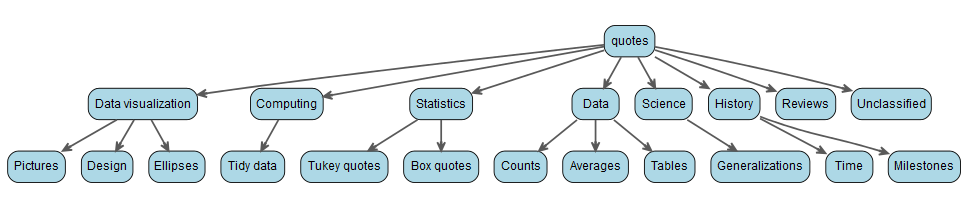
\includegraphics[width=\textwidth]{qtree}
\end{centering}

The exact wording and the attribution (``source'') of quotations is often controversial, either for
the author or location.
The cited source given here is sometimes
supplemented by notes on my sources or further discussion.
A good place to track down problem quotations is \url{http://quoteinvestigator.com}.
%\end{abstract}

%\section{}

%% Data Visualization quotes
%% file:  /home/friendly/Library/Documents/tex/quotes.tex

\section{Data visualization}

\epigraph{You can see a lot, just by looking.}{Yogi Berra}

\epigraph{Did you ever see such a thing as a drawing of a muchness?}{Dormouse, \emph{Alice in Wonderland}}

\epigraph{The critical requirement of an effective graphical display is that it stimulate spontaneous perceptions of \emph{structure} in data.}{S. Smith \emph{et al.}, 1990}

\epigraph{Like good writing, producing an effective graphical display requires an understanding of \emph{purpose}---\emph{what} is to be communicated, and to \emph{whom}.}{Michael Friendly, ``Gallery of Data Visualization'', 1991}

\epigraph{Have you ever seen voice mail?}{\emph{The Hackers Test}}

\epigraph{Graphics is the visual means of resolving logical problems.}{Jacques Bertin \citet[p. 16]{Bertin:81}}

\epigraph{The greatest value of a picture is when it forces us to notice what we never expected to see.}{John W. Tukey \citet[p. vi]{Tukey:77}}

\epigraph{If one technique of data analysis were to be exalted above all others for its ability to be revealing to the mind in connection with each of many different models, there is little doubt which one would be chosen. The simple graph has brought more information to the data analyst's mind than any other device. It specializes in providing indications of unexpected phenomena.}{John W. Tukey \citet[p. 49]{Tukey:1962}}
 
\epigraph{Genius seems to consist merely in trueness of sight.}{Ralph Waldo Emerson, 1840}

\epigraph{The eye obeys exactly the action of the mind.}{Ralph Waldo Emerson, 1860}

\epigraph{Vision is the art of seeing things invisible.}{Johnathan Swift, 1711}

\epigraph{When there is no vision, the people perish.}{Proverbs 29:18}

\epigraph{If I can't picture it, I can't understand it.}{Albert Einstein}

\epigraph{And those who have insight will shine brightly like the brightness of the expanse of Heaven.}{Daniel 12:3}

\epigraph{The one thing that marks the true artist is a clear perception and a firm, bold hand, in distinction from that imperfect mental vision and uncertain truth which give up the feeble pictures and the lumpy statues of the mere artisans on canvas or in stone.}{Oliver Wendell Holmes (1860), \emph{The Professor at the Breakfast Table}, Ticknor and Fields, Boston, MA}

\epigraph{The universe is built on a plan the profound symmetry of which is somehow present in the inner structure of our intellect.} {Paul Valery, 1871--1945}

See: \url{http://www.brainyquote.com/quotes/quotes/p/paulvalery391460.html#PYyvAbp7yY4i1M6w.99}

\epigraph{I like your motto: One picture is worth 1,000 denials.}{Ronald Reagan to White House News Photographers Assn, 18 May 1983}

\epigraph{With brush you paint the possibilities; with pens you scribe the probabilities; for in pictures we find insight; while in numbers find we strength.}{Forrest W. Young}

\epigraph{A graphic should not only show the leaves; it should show the branches as well as the entire tree.}{Jacques Bertin \cite[preface]{Bertin:83}}

\epigraph{Tables are like cobwebs, like the sieve of Danaides; beautifully reticulated, orderly to look upon, but which will hold no conclusion. Tables are abstractions, and the object a most concrete one, so difficult to read the essence of.}{From Chartism by Thomas Carlyle (1840), Chapter II, Statistics}

\epigraph{A judicious man looks at Statistics, not to get knowledge, but to save himself from having ignorance foisted on him.}{Thomas Carlyle, \emph{Chartism}, Chapter II, Statistics}

\epigraph{Although geometrical representations of propositions in the thermodynamics of fluids are in general use and have done good service in disseminating clear notions in this science, yet they have by no means received the extension in respect to variety and generality of which they are capable.}{J. Willard Gibbs, \emph{Graphical Methods in the Thermodynamics of Fluids}, 1873 \citeyear{Gibbs:1873a}}

\epigraph{Although we often hear that data speak for themselves, their voices can be soft and sly.}{Mosteller, Fienberg and Rourke, \emph{Beginning Statistics with Data Analysis}, 1983, Reading MA, p. 234}

\epigraph{Nocturne, of Chopin, so beautiful music. But few people will appreciate the music if I just show them the notes. Most of us need to listen to the music to understand how beautiful it is. But often that's how we present statistics; we just show the notes, we don't play the music.}{Hans Rosling, OECD World Forum, Istanbul, June 2007}

\epigraph{The greatest possibilities of visual display lie in vividness and inescapability of the intended message. A visual display can stop your mental flow in its tracks and make you think. A visual display can force you to notice what you never expected to see.}{John W. Tukey \citeyear{Tukey:90}}

\epigraph{The purpose of [data] display is comparison (recognition of phenomena), not numbers ... The phenomena are the main actors, numbers are the supporting cast.}{John W. Tukey \citeyear{Tukey:90}}

\epigraph{If an editor should print bad English he would lose his position. Many editors are using and printing bad methods of graphic presentation, but they hold their jobs just the same.}{W. C. Brinton, \emph{Graphic methods of presenting facts}, 1914, p. 3}

\epigraph{Around the turn of the century, Karl Pearson, an almost elemental force for more and better statistical thought in all areas of life, including with gusto, matters of social policy, was thinking and lecturing about graphical methods. But later in Pearson's life, and certainly in the careers of R. A. Fisher and the other great statistical minds of the first half of the century, there was a falling away of interest in graphics and an efflorescence  of devotion to analytical mathematical methods. Indeed, for many years there was a contagious \emph{snobbery} against so unpopular, vulgar and elementary a topic as graphics among academic statisticians and their students''}{William Kruskal \citep[p. 144, italics in original]{Kruskal:1978}}



\epigraph{Si la statistique  graphique, bien que  n�e d'hier, �tend  chaque jour son  domaine,  c'est  qu'elle remplace  avantageusement  les  longs tableaux  de chiffres et qu'elle permet, non seulement d'embrasser d'un coup d'oeil la  s�rie des ph�nom�nes, mais  encore d'en signaler  les rapports ou  les anomalies, d'en trouver les causes, d'en d�gager les lois.}{\'Emile Cheysson, c. 1877} 

\epigraph{If statistical graphics, although born just yesterday, extends its reach every day, it is because it replaces long tables of numbers and it allows one not only to embrace at glance the series of phenomena, but also to signal the correspondences or anomalies, to find the causes, to identify the laws.}{\'Emile Cheysson, c. 1877}

\epigraph{Numbers have an important story to tell. They rely on you to give them a clear and convincing voice}{Stephen Few}

\epigraph{Visualizations act as a campfire around which we gather to tell stories}{Al Shalloway}
% from http://blog.fusioncharts.com/2014/05/10-quotes-on-data-visualization/

\epigraph{The purpose of visualization is insight, not pictures}{Ben Shneiderman}


\epigraph{I love taxonomies, categories, ways of dividing people into groups}{Gretchen Rubin}
%See: \url{http://www.brainyquote.com/quotes/keywords/categories_3.html#Ck2SQGKMPjgVJ5Rv.99}

\epigraph{Ballerinas are often divided into three categories: jumpers, turners and balancers}{Robert Gottlieb}

See:\url{http://www.brainyquote.com/quotes/keywords/categories_4.html#JteWy07ipwdTY8jB.99}

\epigraph{There is a magic in graphs. The profile of a curve reveals in a flash a whole situation---the life history of an epidemic, a panic, or an era of prosperity. The curve informs the mind, awakens the imagination, convinces.

Graphs carry the message home. A universal language, graphs convey information directly to the mind. Without complexity there is imaged to the eye a magnitude to be remembered. Words have wings, but graphs interpret. Graphs are pure quantity, stripped of verbal sham, reduced to dimension, vivid, unescapable.

Graphs are all inclusive. No fact is too slight or too great to plot to a scale suited to the eye. Graphs may record the path of an ion or the orbit of the sun, the rise of a civilization, or the acceleration of a bullet, the climate of a century or the varying pressure of a heart beat, the growth of a business, or the nerve reactions of a child.

The graphic art depicts magnitudes to the eye. It does more. It compels the seeing of relations. We may portray by simple graphic methods whole masses of intricate routine, the organization of an enterprise, or the plan of a campaign. Graphs serve as storm signals for the manager, statesman, engineer; as potent narratives for the actuary, statist, naturalist; and as forceful engines of research for science, technology and industry. They display results. They disclose new facts and laws. They reveal discoveries as the bud unfolds the flower.

The graphic language is modern. We are learning its alphabet. That it will develop a lexicon and a literature marvelous for its vividness and the variety of application is inevitable. Graphs are dynamic, dramatic. They may epitomize an epoch, each dot a fact, each slope an event, each curve a history. Wherever there are data to record, inferences to draw, or facts to tell, graphs furnish the unrivalled means whose power we are just beginning to realize and to apply.}{Henry D. Hubbard, in Foreword to \citet{Brinton:1939}, \emph{Graphic Presentation}}
%% graph people vs. table people

\epigraph{Mr. Funkhouser has made an extremely interesting and valuable contribution to the history of statistical method. I wish, however, that he could have added a warning, supported by horrid examples, of the evils of the graphical method unsupported by tables of  figures. Both for  accurate understanding, and particularly to facilitate the use of the same material by other people, it is essential that graphs should not be published by themselves, but only when supported by the tables which lead up to them. It would be an exceedingly good rule to forbid in any scientific periodical the publication of graphs unsupported by tables.}{John Maynard Keynes, review of Funkhouser for \emph{The Economic Journal}, http://www.jstor.org/stable/2224943}

\epigraph{Without data you are just another person with an opinion}{W. Edwards Deming}

\epigraph{Without a plot you are just a person missing a convincing argument}{Di Cook, 2016}
From a review of \emph{Graphical Data Analysis with R}, by Di Cook, JASA, 2016, 111 (514), 912-919

\epigraph{Whatever relates to extent and quantity may be represented by geometrical figures. Statistical projections which speak to the senses without fatiguing the mind, possess the advantage of fixing the attention on a great number of important facts.}{Alexander von Humboldt, \citeyear{Humboldt:1811a}, p. ciii}

\epigraph{Segnius irritant animos demissa per aures, Quam quae sunt oculus subjecta fidelibus (Roughly: What we hear excites the mind less than what we see)}{Horace}

\epigraph{You see, but you do not observe. The distinction is clear.}{Sherlock Holmes, \emph{The Adventures of Sherlock Holmes} (1890), ``A Scandal in Bohemia'', p. 162}

\subsection{Pictures}
\epigraph{Every picture tells a story.}{Rod Stewart, 1971}

\epigraph{A picture is worth a ten thousand words.}{Fred R. Barnard, March 10 1927 in the advertising trade journal \emph{Printers' Ink}}
See: \url{https://en.wikipedia.org/wiki/A_picture_is_worth_a_thousand_words} and \url{http://www2.cs.uregina.ca/~hepting/research/web/words/history.html}

\epigraph{...But it is not always clear \emph{which} 1000 words.}{John W. Tukey, 1973}

\epigraph{Un croquis vaut mieux qu'un long discours. Tr.: A good sketch is better than a long speech.}{Napoleon Bonaparte}

\epigraph{A picture is worth a thousand numbers.}{Anon}

\epigraph{Show me your flowcharts and conceal your tables, and I shall continue to be mystified. Show me your tables, and I won’t usually need your flowcharts; they’ll be obvious.}{Fred Brooks, \emph{The Mythical Man-Month}}

\epigraph{Look here, upon this picture, and on this.}{Shakespeare, Hamlet}


\epigraph{I am only a picture-taster, the way others are wine- or tea-tasters.}{Bernard Berenson, \emph{Sunset and Twilight} Harcourt, Brace \& World, 1963}

\epigraph{Getting information from a table is like extracting sunlight from a cucumber.}{Farquhar \& Farquhar, 1891} % \cite{FaquharFaquhar:1891}

\epigraph{When a law is contained in figures, it is buried like metal in an ore; it is necessary to extract it.  This is the work of graphical representation. It points out the coincidences, the relationships between phenomena, their anomalies, and we have seen what a powerful means of control it puts in the hands of the statistician to verify new data, discover and correct errors with which they have been stained.}{\'Emile Cheysson, \emph{Les m\'ethods de la statistique} (1890), 34-35.}

\subsection{Design}

\epigraph{[When] you see excellent graphics, find out how they were done. Borrow strength from demonstrated excellence.  The idea for information design is: Don't get it original, get it right.}{Edward Tufte}

\epigraph{Good design is obvious. Great design is transparent.}{Joe Sparano, graphic designer for Oxide Design Co.}

\epigraph{Content precedes design. Design in the absence of content is not design, it’s decoration.}{Jeffrey Zeldman, web designer and entrepreneur}

%%%%%%%%%%%%%%%%%%%%%%%%%%%%%%%%%%%%%%%%%%%%%%%%%%%%%%%%%%%%%%%%%%%%%%%%%%%%%%%%%%%%%%%%%%
\subsection{Ellipses}

\epigraph{Mankind is not a circle with a single center but an ellipse with two focal points of which facts are one and ideas the other.}{Victor Hugo}

\epigraph{So, Fabricius, I already have this: that the most true path of the planet [Mars] is an ellipse, which D�rer also calls an oval, or certainly so close to an ellipse that the difference is insensible}{Johannes Kepler, 1605}

Letter to David Fabricius (11 Oct 1605). Johannes Kepler Gesammelte Werke (1937- ), Vol. 15, letter 358, l. 390-92, p. 249.
See: \url{http://www.todayinsci.com/QuotationsCategories/E_Cat/Ellipse-Quotations.htm}


\section{Computing}

\epigraph{Programming graphics in X is like finding the square root of $\pi$ using Roman numerals.}{Henry Spencer}

\epigraph{The purpose of computing is insight, not numbers.}{Richard Hamming, \emph{Introduction To Applied Numerical Analysis}}

\epigraph{... to be a good theoretical statistician one must also compute, and must therefore have the best computing aids.}{Frank Yates, \emph{Sampling Methods for Censuses and Surveys}, 1949}

\epigraph{We [he and Halmos] share a philosophy about linear algebra: we think basis-free, we write basis-free, but when the chips are down we close the office door and compute with matrices like fury.}{Kaplansky, Irving \emph{Paul Halmos: Celebrating 50 Years of Mathematics}}

\epigraph{Seek computer programs that allow you to do the thinking.}{George E. P. Box}

\epigraph{If you only know how to use a hammer, every problem starts to look like a nail.  Stay away from that trap.}{Richard B. Johnson}

\epigraph{[It is] best to confuse only one issue at a time.}{Kernihan \& Ritchie}

\epigraph{The nice thing about standards is that there are so many of them to choose from.}{Andrew Tanenbaum, \emph{Computer Networks}}


%% Tidy, ship-shape
\subsection{Tidy data}
\epigraph{Be careful the environment you choose for it will shape you; be careful the friends you choose for you will become like them.}{W. Clement Stone}

\epigraph{Be careless in your dress if you must, but keep a tidy soul}{Mark Twain}

\epigraph{I'm a tidy sort of bloke. I don't like chaos. I kept records in the record rack, tea in the tea caddy, and pot in the pot box}{George Harrison}

See: \url{http://www.brainyquote.com/quotes/keywords/tidy.html#P43PMcAEC7OxVV3O.99}

%% QUOTES ON STATISTICS -- from http://www.stat.wisc.edu/~limt/quotes
\section{Statistics}

Some of these originally from \url{http://www.stat.wisc.edu/~limt/quotes}

\begin{verse}
Thou shalt not answer questionnaires\\
Or quizzes upon World Affairs,\\
Nor with compliance\\
Take any test. Thou shalt not sit\\
With statisticians nor commit\\
A social science\\
-- W.H. Auden 
\end{verse}

Short version:
\epigraph{Thou shalt not sit with statisticians nor commit a Social Science.}{W.H. Auden}


\epigraph{There are two kinds of statistics, the kind you look up and the kind you make up.}{Rex Stout}

\epigraph{Statistics are like alienists -- they will testify for either side.}{Fiorello H. La Guardia}

\epigraph{You may prove anything by figures.}{Thomas Carlyle}


\epigraph{To understand God's thoughts we must study statistics, for these are the measure of His purpose.}{Florence Nightingale}

\epigraph{You cannot feed the hungry on statistics.}{David Lloyd George}

\epigraph{A single death is a tragedy, a million deaths is a statistic.}{Joseph Stalin}

\epigraph{A judicious man uses statistics, not to get knowledge, but to save himself from having ignorance foisted upon him.}{Thomas Carlyle}

\epigraph{Statistics are like a bikini.  What they reveal is suggestive, but what they conceal is vital.}{Aaron Levenstein}

\epigraph{Do not put faith in what statistics say until you have carefully considered what they do not say.}{William W. Watt}

\epigraph{Facts are stubborn things, but statistics are more pliable.}{Mark Twain}

\epigraph{Statistics are figures used as arguments.}{Leonard L. Levison}

\epigraph{Figures won't lie but liars will figure.}{Charles Grosvenor}

\epigraph{I always find that statistics are hard to swallow and impossible to digest.  The only one I can remember is that if all the people who go to sleep in church were laid end to end they would be a lot more comfortable.}{Mrs Robert A. Taft}

\epigraph{Statistician: Delphic figure who lacks the necessary vocabulary to converse with mere mortals.}{Rod Nicolson, Psychology Software News}

\epigraph{Get the facts first, and then you can distort them as much as you please.}{Mark Twain}

\epigraph{If you want to inspire confidence, give plenty of statistics. It does not matter that they should be accurate, or even intelligible, as long as there is enough of them.}{Lewis Carroll}

\epigraph{It is a truth very certain that when it is not in our power to determine what is true we ought to follow what is most probable.}{Rene Descartes}

\epigraph{Models are to be used, but not to be believed.}{Henry Theill}

\epigraph{A beautiful theory, killed by a nasty, ugly little fact.}{Thomas H. Huxley}

\epigraph{The deepest sin of the human mind is to believe things without evidence.}{Thomas H. Huxley}

\epigraph{Man must learn to simplify, but not to the point of falsification.}{Aldous Huxley}

\epigraph{Do not put your faith in what statistics say until you have carefully considered what they do not say.}{William W. Watt}
	
\epigraph{Since small differences in probability cannot be appreciated by the human mind, there seems little point in being excessively precise about uncertainty.}{Box, G. E. P. \& Tiao, G. C. (1973), \emph{Bayesian inference in statistical analysis}, Addison-Wesley, Reading, MA, p. 65.}

\epigraph{Some people hate the very name of statistics but I find them full of beauty and interest.  Whenever they are not brutalized, but delicately handled by the higher methods, and are warily interpreted,  their power of dealing with complicated phenomena is extraordinary.}{Francis Galton, \emph{Natual Inheritance}, 1889 p. 62}

\epigraph{[Statistics are] the only tools by which an opening may be cut through the formidable thicket of difficulties that bars the path of those who pursue the Science of Man.}{Galton, quoted in K. Pearson, \emph{The Life, Letters and Labours of Francis Galton} (London, 1914)}

\epigraph{Data analysis is an aid to thinking and not a replacement for.}{Richard Shillington}

\epigraph{Sometimes the only thing you can do with a poorly designed experiment is to try to find out what it died of.}{R. A. Fisher}

\epigraph{The best time to plan an experiment is after you've done it.}{R. A. Fisher}

\epigraph{[The War Office kept three sets of figures:] one to mislead the public, another to mislead the Cabinet, and the third to mislead itself.}{Herbert Asquith in Alistair Horne, Price of Glory}

\epigraph{Why are you testing your data for normality?  For large sample sizes the normality tests often give a meaningful answer to a meaningless question (for small samples they give a meaningless answer to a meaningful question)}{Greg Snow, R-Help, 21 Feb 2014}

\epigraph{The relevant question is not whether ANOVA assumptions are met exactly, but rather whether the plausible violations of the assumptions have serious consequences on the validity of probability statements based on the standard assumptions}{Glass et al, 1972, p. 237}
Glass, G. V., Peckham, P. D., \& Sanders, J. R. (1972). Consequences  of failure to meet 
assumptions underlying the fixed effects analyses of variance and covariance.
\emph{Review of Educational Research},  42, 237-288.  


\subsection{Tukey quotes}

\epigraph{Exploratory data analysis can never be the whole story, but nothing else	can serve as the foundation stone -- as the first step.}{John W. Tukey, EDA, 1977, p.3.} 

%% Georges' quotes

\epigraph{The best thing about being a statistician is that you get to play in everyone's backyard.}{John W. Tukey}

\epigraph{Far better an approximate answer to the right question, which is often vague, than an exact answer to the wrong question, which can always be made precise.}{John W. Tukey, (1962), ``The future of data analysis,'' \emph{Annals of Mathematical Statistics}, 33, 1-67.}

\epigraph{A bad answer to a good question may be far better than a good answer to a bad question.}{A graduate class, paraphrasing Tukey's dictum.}

\epigraph{The worst, i.e., most dangerous, feature of 'accepting the null hypothesis' is the giving up of explicit uncertainty ... Mathematics can sometimes be put in such black-and-white terms, but our knowledge or belief about the external world never can.}{John W. Tukey. (1991). ``The Philosophy of Multiple Comparisons,'' \emph{Statistical Science} 6, 100--116.}

\epigraph{Better to have an approximate answer to the right question than a precise answer to the wrong question.}{John W. Tukey as quoted by John Chambers}


\subsection{Box quotes}

\epigraph{All models are wrong but some are useful.}{George E. P. Box, 1979, p 201.}

History of this quote, from : \url{http://en.wikiquote.org/wiki/Talk:George_E._P._Box}

As documented in: Box, George E. P., \emph{J. American Statistical Assoc.}, Vol 74, Number 365, March 1979, ``Some Problems of Statistics of Everyday Life''

An early quote of this idea was: "Models, of course, are never true, but fortunately it is only necessary that they be useful."

The quote ``all models are wrong but some are useful'' is the title of a section of the paper Box, G.E.P. (1979) ``Robustness in the strategy of scientific model building'' in \emph{Robustness in Statistics} (R.L. Launer and G.N. Wilkinson, Eds.), Academic Press. But since this is the proceedings of a meeting that took place in April 11-12 1978, this is likely to be the original quote.

Another reference: Box \& Draper (1987), \emph{Empirical model-building and response surfaces}, Wiley, p. 424.

\epigraph{Every model is an approximation.}{George E. P. Box}



\epigraph{The business of the statistician is to catalyze the scientific learning process.}{George E. P. Box}

\epigraph{Statisticians, like artists, have the bad habit of falling in love with their models.}{George E. P. Box}

\epigraph{If there were a probability of only p = 0.04 of finding a crock of gold behind the next tree, wouldn't you go and look?}{George E. P. Box}

\epigraph{Seek computer programs that allow you to do the thinking.}{George E. P. Box}

\epigraph{When the ratio of the largest to smallest observation is large you should question whether the data are being analyzed in the right metric (transformation).}{George E. P. Box}

\epigraph{A useful type of time series model is a recipe for transforming serial data into white noise.}{George E. P. Box}


\epigraph{It is the data that are real (they actually happened!) The model is a hypothetical conjecture that might or might not summarize and/or explain important features of the data}{George Box}

\epigraph{It is not unusual for a well-designed experiment to analyze itself.}{George Box}

\epigraph{Discovering the unexpected is more important than confirming the known.}{George Box} 



%% Data ----------------------------------------------------

\section{Data}
\epigraph{`Data! data!' he cried impatiently.  I can't make bricks without clay.}{Arthur Conan-Doyle, \emph{Adventures of Sherlock Holmes}, ``The Copper Beeches''}

See: \url{https://en.wikiquote.org/wiki/Sherlock_Holmes}

\epigraph{I have no data yet. It is a capital mistake to theorize before one has data.}{Arthur Conan-Doyle, \emph{Adventures of Sherlock Holmes}, ``A Scandal in Bohemia''}

\epigraph{This was an unexpected piece of luck. My data were coming more quickly than I could have reasonably hoped.}{Arthur Conan-Doyle, \emph{Memoirs of Sherlock Holmes, The Musgrave Ritual}}


\epigraph{I have not all my facts yet, but I do not think there are any insuperable difficulties. Still, it is an error to argue in front of your data. You find yourself insensibly twisting them round to fit your theories.}{Arthur Conan-Doyle, \emph{His Last Bow, Wisteria Lodge}}

\epigraph{It is a capital mistake to theorize before one has data.}{Sherlock Homes in \emph{Scandal in Bohemia}}


\epigraph{The only thing we know for sure about a missing data point is that it is not there, and there is nothing that the magic of statistics can do do change that.  The best that can be managed is to estimate the extent to which missing data have influenced the inferences we wish to draw.}{Howard Wainer, 2009}

\epigraph{Big data can change the way social science is performed, but will not replace statistical common sense.}{Thomas Landsall-Welfare, ``Nowcasting the mood of the nation,'' \emph{Significance}, v. 9(4), August 12, 2012, p. 28} 

\epigraph{Baseball is ninety percent mental and the other half is physical.}{Yogi Berra}

\epigraph{Whenever I see an outlier, I never know whether to throw it away or patent it.}{Bert Gunter quoting a colleague, R-Help, 9/14/2015}
%(Quote from a long ago engineering colleague: "Whenever I see an
%outlier, I never know whether to throw it away or patent it.")
%-- Bert Gunter, R-Help, 9/14/2015

\subsection{Counts}

\epigraph{How do I love thee? Let me count the ways.}{Elizabeth Barrett Browning, \emph{Sonnets from the Portuguese}}

\epigraph{Not everything that counts can be counted, and not everything that can be counted counts.}{Albert Einstein}

\epigraph{Whenever you can, count.}{Francis Galton, quoted in Newman}

\subsection{Averages}

\epigraph{It is difficult to understand why statisticians commonly limit their inquiries to Averages, and do not revel in more comprehensive views. Their souls seem as dull to the charm of variety as that of the native of our flat English counties, whose retrospect of Switzerland was that, if its mountains could be thrown into its lakes, two nuisances would be got rid of at once.}{Francis Galton in \emph{Natural Inheritance}}


\epigraph{Winwood Reade is good upon the subject. He remarks that, while the individual man is an insoluble puzzle, in the aggregate he becomes a mathematical certainty. You can, for example, never foretell what any one man will do, but you can say with precision what an average number will be up to. Individuals vary, but percentages remain constant. So says the statistician.}{Arthur Conan-Doyle, \emph{Sign of the Four}}


\subsection{Tables}

\epigraph{The graphical method has considerable superiority for the exposition of statistical facts over the tabular. A heavy bank of figures is grievously wearisome to the eye, and the popular mind is as incapable of drawing any useful lessons from it as of extracting sunbeams from cucumbers.}{Arthur B. \& Henry Farquhar (1891). Economic and Industrial Delusions \citet[p. 55]{FaquharFaquhar:1891}}


\epigraph{Let it serve for table-talk.}{William Shakespeare. The Merchant of Venice, Act III, Sc. 5.}

%\epigraph{
	\begin{verse}
	While memory holds a seat \\
	In this distracted globe. Remember thee! \\
	Yea, from the table of my memory \\
	I 'll wipe away all trivial fond records. \\
-- William Shakespeare. Hamlet, Act I, Sc. 5.
	\end{verse}
%}{
%}

\epigraph{I drink to the general joy o' the whole table.}{William Shakespeare. Macbeth, Act III, Sc. 4.}

\epigraph{Isolated facts, those that can only be obtained by rough estimate and that require development, can only be presented in memoires; but those that can be presented in a body, with details, and on whose accuracy one can rely, may be expounded in tables.}{E. Duvillard, \emph{M{\'e}moire sur le travail du Bureau de statistique}, 1806; cited in \citet[p. 38]{Derosieres:98}}

 




%% Science --------------------------------------------

\section{Science}

\epigraph{My purpose  is to  set forth  a very  new science  dealing with  a very  ancient subject.  There  is, in  nature, perhaps  nothing older than motion, concerning which the books written by philosophers are neither few nor small;  nevertheless I have discovered by experiment some properties of it which are worth knowing and which have not hitherto been either observed or demonstrated.} {Galileo, \emph{Dialogues and Mathematical Demonstrations Concerning Two New Sciences} (1638)}
See: \url{https://en.wikiquote.org/wiki/Galileo_Galilei}

\epigraph{Study without reflection is a waste of time; reflection without study is dangerous}{Confuscius, Analects (551-479 BC)}

\epigraph{All truths are easy to understand once they are discovered; the point is to discover them}{Galileo} 

\epigraph{Things should be made as simple as possible, but not any simpler}{Albert Einstein}

\epigraph{So much has already been written about everything that you can't find out anything about it.}{James Thurber, 1961}

\epigraph{The practical power of a statistical test is the product of its' statistical power and the probability of use.}{John W. Tukey, 1959 \citep{Tukey:59}}

\epigraph{Theory into Practice.}{Mao Tse-Tung, \emph{The Little Red Book}}

\epigraph{``Beauty is truth; truth, beauty.'' That is all ye know on Earth, and all ye need to know.}{John Keats, \emph{Ode on a Grecian urn}}

\epigraph{They consider me to have sharp and penetrating vision because I see them through the mesh of a sieve.}{Kahlil Gibran}

\epigraph{The journalistic vision sharpens to the point of maximum impact every event, every individual and social configuration; but the honing is uniform.}{George Steiner}

\epigraph{Some people weave burlap into the fabric of our lives, and some weave gold thread. Both contribute to make the whole picture beautiful and unique.}{Anon.}

\epigraph{Time extracts various values from a painter's work. When these values are exhausted the pictures are forgotten, and the more a picture has to give, the greater it is.}{Henri Matisse}

\epigraph{God is in the details.}{Mies van der Rohe, \emph{New York Times}, August 19, 1969}

\epigraph{The devil is in the details.}{George Schultz} % referring to the intracies of the SALT talks in a speech to the Council of Foreign Relations

\epigraph{One has to be able to count if only so that at fifty one doesn't marry a girl of twenty.}{Maxim Gorky, \emph{The Zykovs}, 1914}

\epigraph{A man has one hundred dollars and you leave him with two dollars, that's subtraction.}{Mae West, \emph{My Little Chickadee}, 1940}

\epigraph{In the fields of observation chance favors only the prepared mind.}{Louis Pasteur}

\epigraph{The eye of a human being is a microscope, which makes the world seem bigger than it really is.}{Kahlil Gibran, \emph{A Handful of Sand on the Shore}}

\epigraph{To the man who only has a hammer in the toolkit, every problem looks like a nail.}{Abraham Maslow}

\epigraph{Four hostile newspapers are more to be feared than a thousand bayonets.}{Napoleon Bonaparte, \emph{Maxims}}

\epigraph{When I'm working on a problem, I never think about beauty. I think only how to solve the problem. But when I have finished, if the solution is not beautiful, I know it is wrong.}{Richard Buckminster Fuller}

\epigraph{He who asks a question is a fool for five minutes; he who does not ask a question remains a fool forever.}{Chinese Proverb}

\epigraph{The great tragedy of science -- the slaying of a beautiful hypothesis by an ugly fact.}{Thomas Huxley}

\epigraph{Give a man to fish and he will eat for a day. Teach a man to fish and he will eat for the rest of his life.}{Chinese Proverb}

\epigraph{Give a man a fish and he will eat for a day. Teach a man to fish and you lose a consulting job forever.}{Howard Wainer, 2016}

\epigraph{When you have eliminated the impossible, whatever remains, however improbable, must be the truth.}{Arthur Conan Doyle, \emph{The Sign of the Four} (1890), Ch. 6}

\epigraph{If you choose to represent the various parts in life by holes upon a table, of different shapes---some circular, some triangular, some square, some oblong---we shall generally find that the triangular person has got into the square hole, the oblong into the triangular, and a square person has squeezed himself into the round hole.}{Sydney Smith, 1769-1845}


\epigraph{I know of scarcely anything so apt to impress the imagination as the wonderful form of cosmic order expressed by the ``Law of Frequency of Error.'' The law would have been personified by the Greeks and deified, if they had known of it. It reigns with serenity and in complete self-effacement, amidst the wildest confusion. The huger the mob, and the greater the apparent anarchy, the more perfect is its sway. It is the supreme law of Unreason. Whenever a large sample of chaotic elements are taken in hand and marshaled in the order of their magnitude, an unsuspected and most beautiful form of regularity proves to have been latent all along.}{Sir Francis Galton, \emph{Natural Inheritance}, London: Macmillan, 1889. Quoted in J. R. Newman (ed.) The World of Mathematics, New York: Simon and Schuster, 1956. p. 1482.}

\epigraph{In scientific thought we adopt the simplest theory which will explain all the facts under consideration and enable us to predict new facts of the same kind. The catch in this criterion lies in the world ``simplest.'' It is really an aesthetic canon such as we find implicit in our criticisms of poetry or painting. The layman finds such a law as $dx/dt = K(d^2x/dy^2)$ much less simple than "it oozes," of which it is the mathematical statement. The physicist reverses this judgment, and his statement is certainly the more fruitful of the two, so far as prediction is concerned. It is, however, a statement about something very unfamiliar to the plainman, namely, the rate of change of a rate of change.}{John Burdon Sanderson Haldane (1892--1964) Possible Worlds, 1927.}

\epigraph{Oh, what a tangled web we weave, When first we practice to deceive!}{Sir Walter Scott}

\epigraph{Practice is the best of all instructors.}{Publilius Syrus}

\epigraph{We should go to the masses and learn from them, synthesize their experience into better, articulated principles and methods, then do propaganda among the masses, and call upon them to put these principles and methods into practice so as to solve their problems and help them achieve liberation and happiness.}{Chairman Mao Zedong, "Get Organized!" (November 29, 1943), Selected Works, Vol. III, p. 158.}

\epigraph{The best thing about being a statistician is that you get to play in everyone's backyard.}{John W. Tukey}% from obituary, NY Times, July 28,00/Tukey

\epigraph{An elementary demonstration is one that requires no knowledge--- just an infinite amount of intelligence.}{Richard Feynman}

\epigraph{Science may be described as the art of systematic over-simplification.}{Karl Popper}

\epigraph{Science is like sex: sometimes something useful comes out, but that is not the reason we are doing it.}{Richard Feynman}

\epigraph{Humanists believe that the world has a fixed number of mysteries, so that when one is solved, our sense of wonder is diminished.  Scientists believe that the world has endless mysteries, so that when one is solved, there are always new ones to ponder.}{D. O. Hebb, quoted by Steven Pinker}

\epigraph{Art and science encounter each other when they seek exactitude.}{Etienne-Jules Marey}

AS quoted in Gus Kayafas, ?Estelle Jussim and Harry N. Abrams, Stopping Time: The Photographs of Harold Edgerton (2000), 2

\epigraph{As a rule, the more bizarre a thing is the less mysterious it proves to be.}{Sherlock Holmes,  \emph{The Adventures of Sherlock Holmes} (1892) ``The Red-Headed League''}

\epigraph{Circumstantial evidence is a very tricky thing. It may seem to point very straight to one thing, but if you shift your own point of view a little, you may find it pointing in an equally uncompromising manner to something entirely different.}{Sherlock Holmes, \emph{The Adventures of Sherlock Holmes} (1892) ``The Boscombe Valley Mystery''}
	
% generalizations

\subsection{Generalizations}
\epigraph{The museum spreads its surfaces everywhere, and becomes an untitled collection of generalizations that mobilize the eye.}{Robert Smithson}

\epigraph{In one word, to draw the rule from experience, one must generalize; this is a necessity that imposes itself on the most circumspect observer.}{Henri Poincare, The Value of Science: Essential Writings of Henri Poincare}
% tags: experience, generalizations, necessity, rule, science


See: \url{http://www.brainyquote.com/quotes/keywords/generalizations.html#Gx8sZUeFjuotuIaQ.99}

\epigraph{If I have seen further, it is by standing on the shoulders of giants.}{Sir Isaac Newton, in a letter to Robert Hooke, Feb. 5, 1676}

\epigraph{Few intellectual pleasures are more keen than those enjoyed by a person who, while he is occupied in some special inquiry, suddenly perceives that it admits of a wide generalization, and that his results hold good in previously-unsuspected directions.}{Francis Galton, \emph{North American Review}, \emph{150}, 419-431 (1890)}

\epigraph{The elegance of a theorem is directly proportional to the number of ideas you can see in it and inversely proportional to the effort it takes to see them.}{George Polya}

\epigraph{A mathematician, like a painter or a poet, is a master of pattern. The mathematician's patterns, like the painter's or the poet's, must be beautiful; the ideas, like the colors or the words, must fit together in a harmonious way. ... There is no permanent place in the world for ugly mathematics.}{G. H. Hardy}

\epigraph{An idea which can be used once is a trick. If it can be used more than once it becomes a method.}{George Polya and Gabor Szego}

%%% Multiple discoveries / Stigler's Law

\epigraph{When the time is ripe for certain things, these things appear in different places in the manner of violets coming to light in early spring.}{Farkas Bolyai to his son J�nos Bolyai, urging him to claim the invention of non-Euclidean geometry without delay, quoted in Ming Li and Paul Vitanyi, An introduction to Kolmogorov Complexity and Its Applications, 1st ed., 1993, p. 83.}


%% tables
%% Averages
\section{History}
\epigraph{The only new thing in the world is the history you don't know.}{Harry S. Truman, quoted by David McCulloch}

\epigraph{So we beat on, boats against the current, borne back ceaselessly into the past.}{F. Scott Fitzgerald, \emph{The Great Gatsby} (1925)}

\epigraph{Euclid alone has looked on beauty bare.}{Edna St Vincent Millay}

\epigraph{The past only exists insofar as it is present in the records of today. And what those records are is determined by what questions we ask.  There is no other history than that.}{Wheeler, 1982:24}

\epigraph{A generation which ignores history has no past and no future}{Robert Heinlein} % (1907 - 1988), The Notebooks of Lazurus Long


\epigraph{History will be kind to me for I intend to write it.}{Winston Churchill}

\epigraph{For my part, I consider that it will be found much better by all parties to leave the past to history, especially as I propose to write that history myself.}{Winston Churchill}

\epigraph{If you would understand anything, observe its beginning and its development.}{Aristotle}

\epigraph{God alone knows the future, but only an historian can alter the past.}{Ambrose Bierce}

\epigraph{Since God himself cannot change the past, he is obliged to tolerate the existence of historians.}{Attributed to Samuel Butler}

\epigraph{At the heart of good history is a naughty little secret: good storytelling.}{Stephen Schiff}

\epigraph{It has been said that though God cannot alter the past, historians can; it is perhaps because they can be useful to Him in this respect that He tolerates their existence.}{Samuel Butler, \emph{Erewhon Revisted}}

\epigraph{History is moving statistics and statistics is frozen history.}{A. L. Schl\"ozer, \emph{Theorie der Statistik}, 1804, p. 86}


\subsection{Time}

\epigraph{Time flies like an arrow; fruit flies like a banana.}{Anthony G. Oettinger; often mis-attributed to Groucho Marx}

\epigraph{How did it get so late so soon? }{Dr. Seuss}

\epigraph{Time is the longest distance between two places.}{Tennessee Williams, \emph{The Glass Menagerie}}

\epigraph{Those who make the worst use of their time are the first to complain of its brevity.}{Jean de La Bruy�re, Les Caract�res }

%\subsection{Past, present, future}

\epigraph{The past is a foreign country: they do things differently there.}{L. P. Hartley, \emph{The Go-Between}}

\epigraph{I never think of the future - it comes soon enough.}{Albert Einstein}
See: \url{http://quoteinvestigator.com/2013/07/23/future-soon/}

\epigraph{The best way to predict the future is to invent it}{Alan Kay}

\epigraph{Prediction is very difficult, especially about the future}{Niels Bohr}

\epigraph{The future ain't what it used to be}{Yogi Berra}

\epigraph{Look not mournfully into the past. It comes not back again.  Wisely improve the present. It is thine. Go forth to meet the shadowy future, without fear.}{Henry Wadsworth Longfellow} % (1807 - 1882)

\epigraph{Let him who would enjoy a good future waste none of his present.}{Roger Babson}

\epigraph{When in doubt, predict that the present trend will continue.}{Merkin's Maxim}

\epigraph{The only use of a knowledge of the past is to equip us for the present. The present contains all that there is. It is holy ground; for it is the past, and it is the future.}{Alfred North Whitehead} % (1861 - 1947)

\epigraph{My past is my wisdom to use today. ... my future is my wisdom yet to experience. Be in the present because that is where life resides.}{Gene Oliver, Life and the Artistry of Change}

\epigraph{I have realized that the past and future are real illusions, that they exist in the present, which is what there is and all there is.}{Alan Watts}

\epigraph{The future is uncertain but the end is always near.}{Jim Morrison}

\epigraph{Time has no divisions to mark its passage, there is never a thunder-storm of blare of trumpets to announce the beginning of a new month or year. Even when a new century begins, it is only we mortals who ring bells and fire off pistols.}{Thomas Mann, \emph{The Magic Mountain} (1924)}

\subsection{Milestones}

\epigraph{Direction is more important than speed. We are so busy looking at our speedometers that we forget the milestone.}{Anonymous}

\epigraph{Only sixteen players have hit fifty or more homers in a season. To me, that's a very special milestone.}{Mark McGwire}

\epigraph{As life runs on, the road grows strange with faces new -- and near the end. The milestones into headstones change, Neath every one a friend.}{James Russell Lowell}

\section{Reviews}
\epigraph{This paper contains much that is new and much that is true. Unfortunately, that which is true is not new and that which is new is not true.}{attributed to Wolfgang Pauli}

\epigraph{This book fills a much-needed gap.}{Attributed to many}

For the history of this quote and discussion:
\url{http://quoteinvestigator.com/2010/05/03/fills-a-much-needed-gap-pt1/}, 
\url{http://quoteinvestigator.com/2010/05/03/fills-a-much-needed-gap-pt2/}

\epigraph{Russell left the vast darkness of the topic unobscured}{Alfred North Whitehead, referring to Bertrand Russell}

Quote history, from: \url{http://todayinsci.com/QuotationsCategories/U_Cat/Unobscured-Quotations.htm}:
Bertrand Russell had given a talk on the then new quantum mechanics, of whose wonders he was most appreciative. He spoke hard and earnestly in the New Lecture Hall. And when he was done, Professor Whitehead, who presided, thanked him for his efforts, and not least for `leaving the vast darkness of the subject unobscured.' 
Quoted in Robert Oppenheimer, \emph{The Open Mind} (1955), p. 102. 


\section{Unclassified}


\epigraph{Mathematicians have always been rather of a jealous nature, and undoubtedly jealousy was a family characteristic of the Bernoullis.  There is some excuse for mathematicians, for their reputation stands for posterity largely not on what they did, but on what their contemporaries attributed to them.}{Karl Pearson, ``The History of Statistics in the 17th and 18th Centuries'' \cite[p. 226]{Pearson:1978}}

\epigraph{When choosing between two evils, I always like to take the one I've never tried before.}{Mae West, 1941}

\epigraph{To err is human---but it feels divine!}{Mae West}

\epigraph{Good judgment comes from experience; experience comes from bad judgment.}{Fred Brooks}


\epigraph{One must learn by doing the thing; for though you think you know it, you have no certainty until you try.}{Sophocles}


	



\bibliography{graphics,statistics,timeref}


\end{document}
